\documentclass[compress]{beamer}

\usepackage[utf8]{vntex}
\usepackage{longtable}
\usepackage{amsmath}
\usepackage{amsmath}
\usepackage{amsfonts}
\usepackage{amssymb}
\usepackage[utf8]{inputenc}
\usepackage[absolute,overlay]{textpos}

\usepackage{listings}
\lstset{
	language = Java,
	frame = single,
	tabsize = 3
}

\usetheme{Warsaw}
%\usetheme{Antibes}
%\usecolortheme{spruce}
%\setbeamercolor{structure}{fg=cyan!90!blue}

\expandafter\def\expandafter\insertshorttitle\expandafter{%
    \insertshorttitle\hfill%
    \insertframenumber\,/\,\inserttotalframenumber}
      
\AtBeginSection[] % Do nothing for \section*
{
\begin{frame}
\tableofcontents[currentsection]
\end{frame}
}
\AtBeginSubsection[] % Do nothing for \section*
{
\begin{frame}
\tableofcontents[currentsection, currentsubsection]
\end{frame}
}

\title[Mạng Google Inception]{Mạng Google Inception trong bài toán phân loại} 

\author[Nguyễn Tuấn Đạt, Đặng Quang Trung, Phan Anh Tú]{
Sinh viên thực hiện\\
Nguyễn Tuấn Đạt - 20130856\\
Đặng Quang Trung - 20134145\\
Phan Anh Tú - 20134501 \\[0.4cm]
Giảng viên \\
TS. Đinh Viết Sang 
}

\begin{document} 
\begin{frame}
\titlepage
\end{frame} 

\begin{frame}{Phân công công việc}

\end{frame}
  
   
\begin{frame}{Nội dung trình bày}
\tableofcontents
\end{frame}
\begin{frame}{Mạng neuron nhân tạo}
\begin{itemize}
\item Mạng neuron nhân tạo là một mô hình tính toán mô phỏng các hệ thống tương tự mạng neuron sinh học.
\item Mỗi neuron thực hiện một tính toán cục bộ nhận đầu vào và đưa ra đầu ra tương ứng
\item  Chức năng của một  mạng neuron được xác định bởi :
\begin{itemize}
\item Kiến trúc
\item Đặc tính vào ra
\item Chiến lược học
\item Dữ liệu học 
\end{itemize}
\end{itemize}
\end{frame}
\begin{frame}{Học sâu}
Học sâu là một nhánh của học máy trên cơ sở một tập các thuật toán nhằm cố gắng mô hình hóa trừu tượng mức cao trong dữ liệu bởi việc sử dụng với nhiều tầng xử lý. \\
\begin{figure}[H]
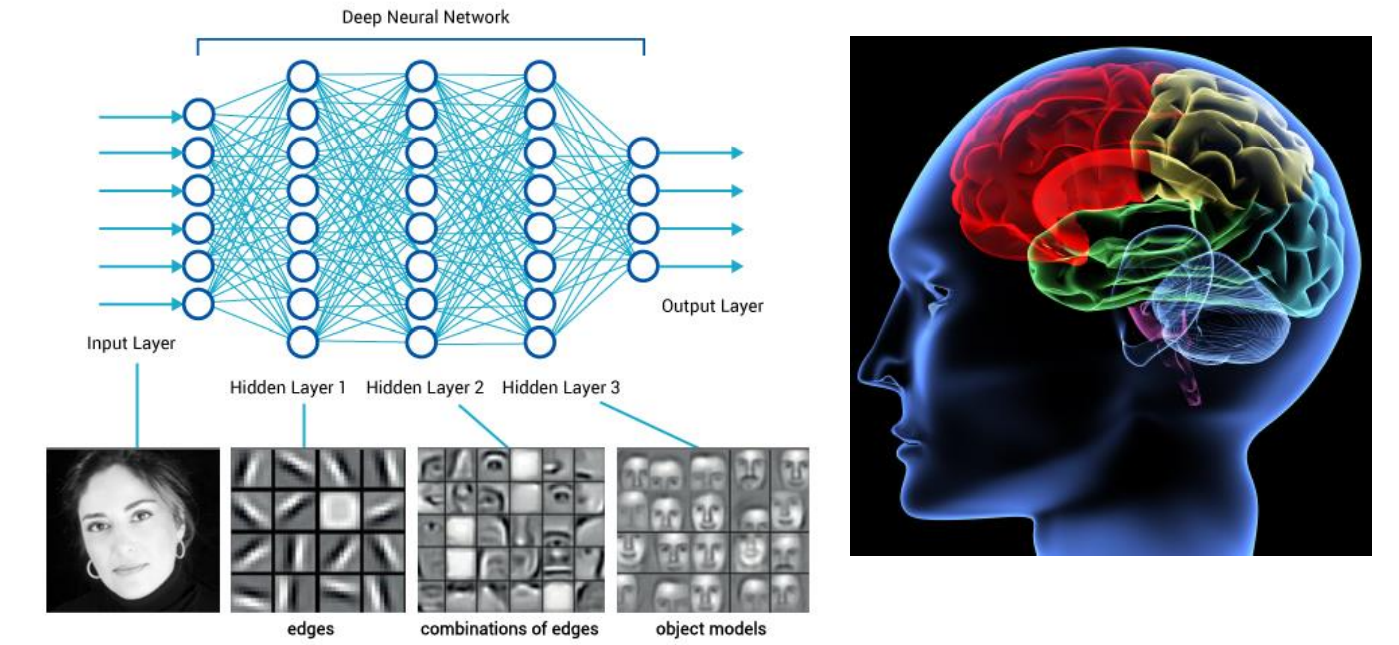
\includegraphics[scale=0.3]{deeplearning.png}
\caption{Mô tả mô hình một mạng neuron học sâu}
\end{figure}
\end{frame}
\begin{frame}{Các thành phần quang trọng trong một mô hình học sâu} 
Hàm mục tiêu:\\ Các hàm mục tiêu hay được sử dụng \begin{itemize}
\item sigmoid $\sigma =1/(1+e^-x)$
\item tanh $ tanh(x)$
\item ReLU $ max(0,x)$
\item ELU \abovedisplayskip=0pt\relax
\begin{equation}
\begin{cases}
x \qquad \qquad \qquad  if x>0\\ \alpha (exp(x)-1) \quad if x \leq 0
\end{cases}
\end{equation}
\item Maxout $max(w_1^T x+b_1,w_2^T x+b_2) $

\end{itemize}

\end{frame}
\begin{frame}{Các thành phần quang trọng trong một mô hình học sâu}
Kiến trúc mạng
\begin{figure}[H]
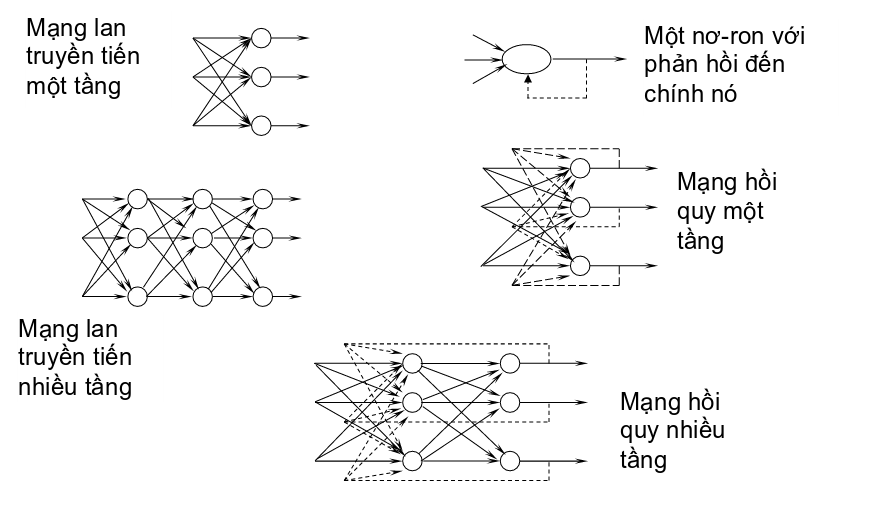
\includegraphics[scale=0.3]{archneuron.png}
\caption{Các kiến trúc mạng neuron điển hình}
\end{figure}
\end{frame}
\begin{frame}{Các thành phần quang trọng trong một mô hình học sâu}
\textbf{Thuật toán học}: Với một mạng neuron lan truyền tiến, hiện tại thuật toán lan truyền ngược vẫn là thuật toán được sử dụng rộng rãi và đem lại hiệu quả cao.\\

\textbf{Chiến lược học}:
\begin{itemize}
\item Stochastic Gradient Descent
\item Mini-batch Gradient Descent
\item SGD-Momentum
\item SGD-Vanilla
\item Adagrad
\item AdaDelta
\end{itemize}

\end{frame}
\begin{frame}{Mạng tích chập}
\begin{itemize}
\item Mạng tích chập là một mạng neuron nhân tạo nhiều tầng. Nhưng điều khác biệt chính là ở mỗi neuron trong tầng ẩn của CNN sẽ không kết nối với toàn bộ các neuron thuộc tầng liền trước như mạng thông thường.
\item Trong kiến trúc CNN gồm 3 tầng chính đó là: Convolution Layer, Pooling Layer, Fully-connected Layer.
\end{itemize}



\end{frame}
\begin{frame}{Convolution Layer}
Tầng CONV sử dụng một tập các bộ lọc. Mỗi bộ lọc là một không gian nhỏ chiều rộng và chiều cao là các tham số cần chọn, trên toàn bộ chiều sâu của khối đầu vào. Mỗi một bộ lọc sẽ trượt trên toàn kích thước mặt của khối đầu vào và tính toán tại vị trí tương ứng mà bộ lọc trượt qua.
\begin{figure}[H]
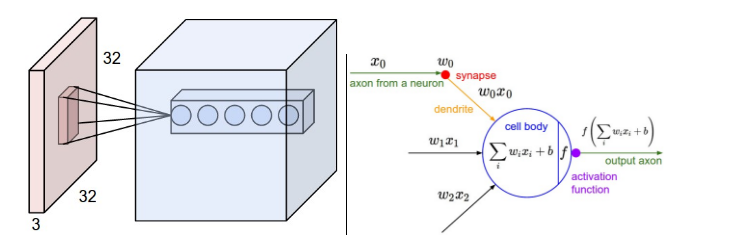
\includegraphics[scale=0.5]{img2.png}
\caption{CONV Layer}
\end{figure}

\end{frame}
\begin{frame}{Convolution Layer}
\begin{itemize}
\item	Không gian số lượng các neurons ở đầu ra được quy định bởi 3 tham số :depth(độ sâu), stride(bước trượt) và mức lề (zero-padding):
\begin{itemize}
\item[1. ] Độ sâu ở đầu ra tương ứng với số lượng bộ lọc được sử dụng.
\item[2. ] Stride là số bước nhảy khi trượt bộ lọc.
\item[3. ] Dữ liệu ở mép các ma trận rất dễ bị mất  dần qua mỗi tầng vì vậy sử dụng một kích thước lề bao quanh đầu vào, giá trị của lề đều bằng 0. 

\end{itemize} 
\item Trong mạng CNN ta luôn chỉ sử dụng một vector trọng số cho các neuron có cùng độ sâu.
\end{itemize}
\end{frame}
\begin{frame}{Ví dụ}
\begin{figure}[H]
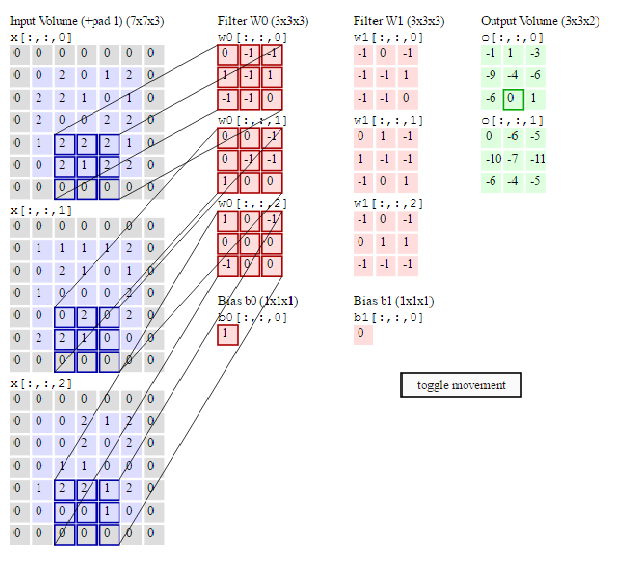
\includegraphics[scale=0.5]{img3.png}
\caption{Ví dụ CONV}
\end{figure}
\end{frame}
\begin{frame}{Pooling Layer}
\begin{figure}[H]
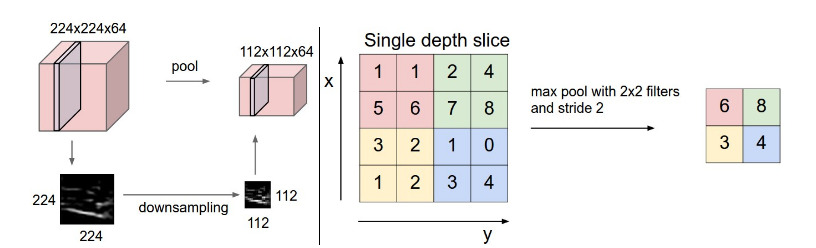
\includegraphics[scale=0.5]{img4.png}
\caption{Ví dụ CONV}
\end{figure}
\end{frame}
\begin{frame}{Kiến trúc CNN}
\small{
\textbf{INPUT -> [[CONV -> RELU]*N -> POOL?]*M -> [FC -> RELU]*K -> FC}
}

\end{frame}
\end{document}
